\documentclass[12pt, a4paper]{article}
\setcounter{tocdepth}{2}
\usepackage{graphicx} % Required for inserting images
\usepackage[parfill]{parskip} % Removes indent from new paragraphs
\usepackage{amsmath, amssymb, amsfonts}
\usepackage[colorlinks = true,
			citecolor  = blue]{hyperref}

\usepackage[longnamesfirst,authoryear, round]{natbib}
\bibliographystyle{unsrtnat}

\usepackage[
top    = 1.0in,
bottom = 1.2in,
left   = 1.0in,
right  = 1.0in]{geometry}
\linespread{1.5}

\title{Comparison of MCMC algorithms in Stochastic Volatility Models}
\author{Benjamin Wee}
\date{October 2023}

\begin{document}

\maketitle 

\begin{abstract}.  
    The objective of this research is to compare the computational methods used to estimate Bayesian stochastic volatility models. A simulation study will compare the estimation strategies detailed in the stochastic volatility literature with Hamiltonian Monte Carlo and their ability to sample from the model's posterior distribution. Specifically, Simulation Based Calibration (SBC) is used to check whether these sampling strategies are returning efficient and well calibrated posterior estimates. Key metrics of interest are the effective sample size to check the efficiency of the algorithm and tests of uniformity to assess the calibration of the posteriors. This will determine which algorithm is better at estimating stochastic volatility models based on the efficiency and accuracy of the sampling strategy.
\end{abstract}

\newpage

\tableofcontents{\protect\newpage}

\section{Introduction}

- Should make reference to workflow, and reparameterisation of SV.

\section{Background and Literature Review}

    \subsection{Stochastic Volatility}
        Stochastic volatility models are used in financial econometrics to model the variance or volatility of returns in a financial instrument. The return of a financial asset often exhibits patterns in the variance which can be modelled to improve prediction and estimates of risk or tail events. Unlike other volatility models such as ARCH or GARCH, stochastic volatility models treat the variance as a random variable. Furthermore, these models have a state space representation since the variance is expressed as a latent stochastic process. State space models can be difficult to estimate since there is a latent state for every data observation in the time series, which means there are often more parameters than data points. These models can be estimated using frequent frameworks but this research will focus on Bayesian estimation strategies.

        \citet{kim1998stochastic} estimate a discrete time, univariate stochastic volatility model using Bayesian methods which is outlined below. $y_t$ is the mean corrected returns of some asset for equally spaced intervals t. $\beta$ is a constant scaling factor which is also defined as $exp(\mu / 2)$ representing instantaneous volatility. $h_t$ is log volatility, where $h_1$ is a draw from a stationary distribution and the state equation $h_{t+1}$ follows a stationary process governed by the autoregressive parameter $\phi$ such that $|\phi|<1$. This autoregressive parameter represents the persistence or "stickiness" of log volatility and the dispersion parameter $\sigma_{\eta}$ is the constant variance of the states. $\epsilon_t$ and $\eta_t$ are standard normal white noise shocks and are uncorrelated with each other. 

        $$
        \begin{aligned}
        y_t =& \space \beta exp(h_t/2) \epsilon_t \\
        h_{t+1} =& \space \mu +\phi(h_t - \mu) + \sigma_{\eta} \eta_t  \\
        h_1 \sim& \space normal\left(\mu, \frac{\sigma_{\eta}^2}{1-\phi^2}\right) \\
        \end{aligned}
        $$


        $$
        \begin{aligned}
        \epsilon_t \sim& \space normal(0,1) \\
        \delta_t \sim& \space normal(0,1)
        \end{aligned}
        $$

        Setting $\beta=1$, the model can be expressed more succinctly as:

        $$
        \begin{aligned}
        y_t \sim& \space normal(0, exp(h_t/2)) \\ 
        h_1 \sim& \space normal \left(\mu, \frac{\sigma_{\eta}^2}{1-\phi^2}\right) \\
        h_{t+1} \sim& \space normal(\mu +\phi(h_t - \mu) , \sigma_{\eta}^2), \space\space t\neq 1\\ 
        \end{aligned}
        $$

        Priors for the static parameters are defined below with conjugate priors on $\mu$ and $\sigma^2$:

        $$
        \begin{aligned}
        \mu \sim& \space normal(0, 10^2) \\
        \sigma_{\eta}^2 \sim& \space IG(5/2, (0.01\times 5) / 2) \\
        \phi^{\ast} \sim& \space beta(20, 1.5) \\
        \phi &=  2\phi^{\ast} - 1
        \end{aligned}
        $$

        The prior on $\phi$ is a "stretched" beta distribution. This is a beta distribution (as defined on the parameter $\phi^*$) which has been transformed to have support (-1, 1).

    \subsection{Gaussian Mixture Approximation}
        Kim, Shephard and Chib (KSC) sample the posteriors of the stochastic volatility model using a mix of conjugate posterior distributions, Metropolis Hastings and the Kalman Filter and smoother\footnote{In this research the exact software to apply the simulation smoother is unavailable, so a more recent simulation smoother is used which is based on the software written by the same author.} \citep{dejong1995}.

        The standard Kalman Filter and smoother is used to compute the posterior distribution over the latent states. This requires the state and measurement equations to be linear and conditionally Gaussian. Since the relationship between $y_t$ and $h_t$ in the measurement equation is not linear, a transformation is applied by squaring and taking the log of $y_t$.

        $$
        \begin{aligned}
        y_t^{*} &= log(y_t^2) \\ 
        &= log((\epsilon_t exp(h_t/2))^2) \\
        &=  log(exp(h_t)) + log(\epsilon_t^2) \\
        &= h_t + log(\epsilon_t^2)  \\
        &= h_t + z_t \\
        \end{aligned}
        $$

        Where $z_t = log(\epsilon_t^2)$ follows a log chi-squared distribution with mean -1.2704 and variance 4.93. The relationship between $y_t$ and $h_t$ is now linear; however, the error is not Gaussian. Since it is not simple to sample from this parameterisation of the model, KSC use a mixture of Gaussians to **approximate** the first 4 moments of the log chi squared distribution. This is defined by:

        $$
        \begin{aligned}
        f(z_t) = \sum_{i=1}^{K} q_if_N(z_i|m_i-1.2704, \nu_i^2)
        \end{aligned}
        $$

        Where K is the mixture of normal densities $f_N$, component probabilities $q_i$, mean $m_i-1.2704$ and variance $\nu_i^2$. These parameters were selected using moment matching where they found 7 normal densities with varying mean and variance parameters best approximated the log chi squared moments. These parameters and weights can be found in Appendix A.

        The model can be sampled via the Kalman Filter and simulation smoother since the model is now linear and conditionally gaussian. The static parameters $\mu$ and $\sigma^2$ are sampled directly from their conjugate posterior distributions whereas $\phi$ is sampled via a Metropolis Hastings accept/reject procedure. The details can be around in Appendix B. 

    \subsection{Hamiltonian Monte Carlo}
        Since the paper was written, new MCMC algorithms have been developed and enabled the estimation of richer and more complicated models. Specifically, Hamiltonian Monte Carlo is a MCMC algorithm which has become widely available for efficiently sampling from sophisticated models. Hamiltonian Monte Carlo, originally called Hybrid Monte Carlo, was developed in the physics literature \citep{duane1987hybrid} before being applied in the statistics literature by Radford Neal through his works in Bayesian Neural Networks \citep{neal1995bayesian} and statistical computing \citep{neal2011mcmc}. The algorithm has since become widely available through open source development projects such as Stan \citep{stan} and PyMC \citep{pymc2023}.

        The key innovation of Hamiltonian Monte Carlo is using the gradients of the target posterior distribution to generate an efficient path for the sampler to explore. Unlike Random Walk Metropolis Hastings, it takes advantage of the geometry of the posterior to determine its next proposal step. A comprehensive explanation of the sampler is beyond the scope of this research and can be found in the above references. 

        The Stan programming language's implementation of Hamiltonian Monte Carlo will be used for this study. Stan's default algorithm, the No-U-Turn Sampler \citep{hoffman2014no}, allows for direct sampling of the specified stochastic volatility model. Hamiltonian Monte Carlo allows for sampling of the generative model and can flexibly handle complicated likelihood functions. This approach will also use the same priors as specified in the Gaussian mixture approximation.


\section{Methodology}

    \subsection{Simulation Design}
        Simulation Based Calibration (SBC) is a technique that checks the calibration of posterior estimates generated by MCMC algorithms. SBC is conducted by comparing the distribution of rank statistics to the discrete uniform distribution which arises when an algorithm is correctly calibrated. The procedure starts by taking draws from the prior distribution and creating datasets implied by each draw. Rank statistics are then calculated on the posterior samples conditional on the simulated data. 

        To illustrate this procedure, let $\theta$ be a parameter and $y$ represent the dataset. Start with a single draw from the prior distribution:
        
        $$
        \begin{aligned}
        \theta^{sim} \sim \pi(\theta)
        \end{aligned}
        $$

        Generate a dataset given by the prior draw.

        $$
        \begin{aligned}
        y^{sim} \sim \pi (y|\theta^{sim})
        \end{aligned}
        $$

        Then take draws from the posterior distribution generated by a MCMC algorithm or estimation strategy (Hamiltonian Monte Carlo or KSC) conditional on this dataset.

        $$
        \begin{aligned}
        \{\theta_1,\dots , \theta_{L}\} \sim \pi (\theta | y^{sim})
        \end{aligned}
        $$

        A key result is that the posterior sample $\{\theta_1,\dots , \theta_{L}\}$ will share the same distribution as the prior samples $\theta^{sim}$. This is implied by the following expression:

        $$
        \begin{aligned}
        \pi(\theta) &= \int \pi(\theta|y^{sim}) \pi(y^{sim}|\theta^{sim}) \pi(\theta^{sim})dy^{sim} d\theta^{sim} \\
        &= \int \pi(\theta|y^{sim}) \pi(y^{sim},\theta^{sim}) dy^{sim} d\theta^{sim}
        \end{aligned}
        $$

        That is, the posterior averaged over the joint distribution follows the same distribution as the prior. The procedure of generating posterior samples implicitly performs this integral since the expression on the right of the integral is proportional to the prior density. Therefore, any deviation of the posterior samples from the prior distribution suggests that the sampling methodology is not producing the correct posteriors.

        If the posterior samples follows the prior distribution, the rank statistic for a given parameter follows a discrete uniform distribution\footnote{Proof of this result in \citet{talts2018validating}.}. The rank statistic is defined as:

        $$
        \begin{aligned}
        r = rank(\{\theta_1,\dots , \theta_{L}\}, \theta^{sim}) = \sum_{l=1}^{L}1[\theta_{l} < \theta^{sim}]
        \end{aligned}
        $$

        This completes one iteration of SBC. To complete the algorithm, multiple iterations are run and the rank statistics are calculated for each parameter. The resulting rank statistics are compared to the discrete uniform distribution to determine if any problematic features exist.

        If the computation is well calibrated and the rank statistics follow a discrete uniform distribution, then the posterior credible intervals have sufficient coverage. That is, one way to describe calibration is: for any percentage interval selected over the posterior samples (for example 90\%) then there is a 90\% chance that $\theta^{sim}$ falls within this interval. Another way of saying this is a Bayesian analysis is well calibrated if a 90\% credible interval contains the true parameter in 90\% of the SBC iterations. 

    \subsection{Metrics}
        The key metrics and diagnostics to compare the performance of these methods are the effective sample size (ESS), rank statistics, and chi-squared test statistics. 

        ESS measures the efficiency of the MCMC sampler. It calculates the number of effectively independent draws from the posterior draws generated by a Markov chain. A poor ESS can arise from high autocorrelation in the Markov chain which leads to highly dependent samples. An efficient MCMC algorithm takes less resources (for example, time and number of draws) to get a representative sample of the target distribution. If a MCMC algorithm possesses higher ESS for the majority of its parameters (relative to another strategy), then we may conclude that this method is a more efficient sampler (conditional on the model). 
    
        Rank statistics as described in the SBC section are used to evaluate the calibration of a posterior. Histograms will be used to evaluate the distribution of rank statistics. If a posterior is well calibrated then it is expected that the histogram is uniform.
    
        A drawback of this approach is there are more parameters than data points in this model. An alternative to visually checking for uniformity of all the parameters is to calculate the chi squared statistics for the counts in each histogram bin. Let $b_j$ be the number of counts and $e_j$ the expected count in bin $j$. Then the chi squared statistic is given by:
    
        $$
        \begin{aligned}
        \chi^2 = \sum_{j=1}^J \frac{(b_{j} - e_{j})^2}{e_j}
        \end{aligned}
        $$
    
        Chi squared statistics can be used to test for uniformity and thus calibration of all the parameters in the model.
    
    \subsection{Model Parameterisation}

        The parameterisation of a model can affect the performance of a MCMC algorithm when sampling from models with complex posterior geometries. An example of this is Neal's funnel \citep{neal2003slice} where the Hamiltonian Monte Carlo sampler encounters performance issues in hierarchical models and produces biased samples. 

        The stochastic volatility model as described in section 2.1 is follows a "centered" parameterisation. This describes the central location of the latent state parameters which are centered around the mean and lag of the log volatility $\mu +\phi(h_t - \mu)$. A model can be reparameterised such that the states are sampled on a distribution centered on 0 (i.e "non centered") which are later transformed to have the correct mean.  It is useful to compare model parameterisations since sampling strategies may be sensitive to the posterior geometry. 
        
        \subsubsection{Non centered Hamiltonian Monte Carlo}
        First sample from a standard normal distribuition and multiply by the variance of the log volatility.

        $$
        \begin{aligned}
        h_{std} \sim& \space normal(0,1) \\
        h =& h_{std} \times \sigma_{\eta} \\ 
        h \sim& normal(0, \sigma_{\eta}^2)
        \end{aligned}
        $$
        
        The states are sampled with the mean centered at zero. Then apply the appropriate rescaling to get samples from the log volatility. 
        
        $$
        \begin{aligned}
        h_1 =& \space \frac{h_{std, 1}\times \sigma_{\eta}} {\sqrt{1 - \phi^2}} + \mu \\
        h_{t+1} =& \space h_{std, t+1}\times \sigma_{\eta} + \mu  + \phi(h_{t} - \mu),\space t\neq 1
        \end{aligned}
        $$
        
        This returns log volatility as desired.
        
        $$
        \begin{aligned}
        h_1 \sim& \space normal \left(\mu, \frac{\sigma_{\eta}^2}{1-\phi^2}\right) \\
        h_{t+1} \sim& \space normal(\mu +\phi(h_t - \mu) , \sigma_{\eta}^2), \space\space t\neq 1\\ 
        \end{aligned}
        $$

        \subsubsection{Non centered Gaussian Mixture}
        The non centered model for the Gaussian approximation is expressed slightly differently due to the use of the Kalman Filter. While HMC can sample from the joint posterior directly with state vectors centered at zero, applying the Kalman Filter requires the state equation to be a function of the state variable. 

        Starting with the log chi squared model:

        $$
        \begin{aligned}
        y^{\ast}_t =& h_t + z_t \\
        h_{t+1} =& \space \mu +\phi(h_t - \mu) + \sigma_{\eta} \eta_t
        \end{aligned}
        $$
        
        Expand the state equation:
        
        $$
        \begin{aligned}
        h_{t+1} =& \space \mu +\phi(h_t - \mu) + \sigma_{\eta} \eta_t  \\
        =& \space \mu + \phi h_t - \phi\mu + \sigma_{\eta} \eta_t  \\
        =& \space \mu (1- \phi) + \phi h_t + \sigma_{\eta} \eta_t  \\
        \end{aligned}
        $$
        
        Take out the intercept and put it in the measurement equation:
        
        $$
        \begin{aligned}
        y^{\ast}_t =& h_t + \mu (1- \phi) + z_t \\
        h^{\ast}_{t+1} =& \space \phi h_t + \sigma_{\eta} \eta_t  \\
        \end{aligned}
        $$
        
        The mean of the log volatility is now inside the measurement equation and de-meaned from the state equation.

        \subsubsection{Prior Predictive check}
        It is worth noting that the centered and non-centered parameteristions are the same stochastic volatility model. Different parameteristions express the same mathematical models in ways that may make it easier or harder for a given algorithm to sample. 

        To demonstrate this, a prior predictive simulation of the second state parameter is performed for both a centered and non centered model (using the paramterisation described in section 3.3.1). This is the same as the first two steps of SBC, except instead of generating a dataset, generate the parameters implied by the prior draw. Let $\boldsymbol{\theta}$ be a vector of static parameters.

        $$
        \begin{aligned}
        \boldsymbol{\theta}^{sim} \sim \pi(\boldsymbol{\theta})
        \end{aligned}
        $$

        Generate a the second state parameter implied by the joint prior.

        $$
        \begin{aligned}
        h_2^{sim} \sim \pi (h_2|h_1, \boldsymbol{\theta}^{sim})
        \end{aligned}
        $$

        Generating 1000 samples of $h_2^{sim}$ from both centered and non-centered models gives samples from the same data generating process as shown in figure x. 


        % \begin{figure}
        %     \centering
        %     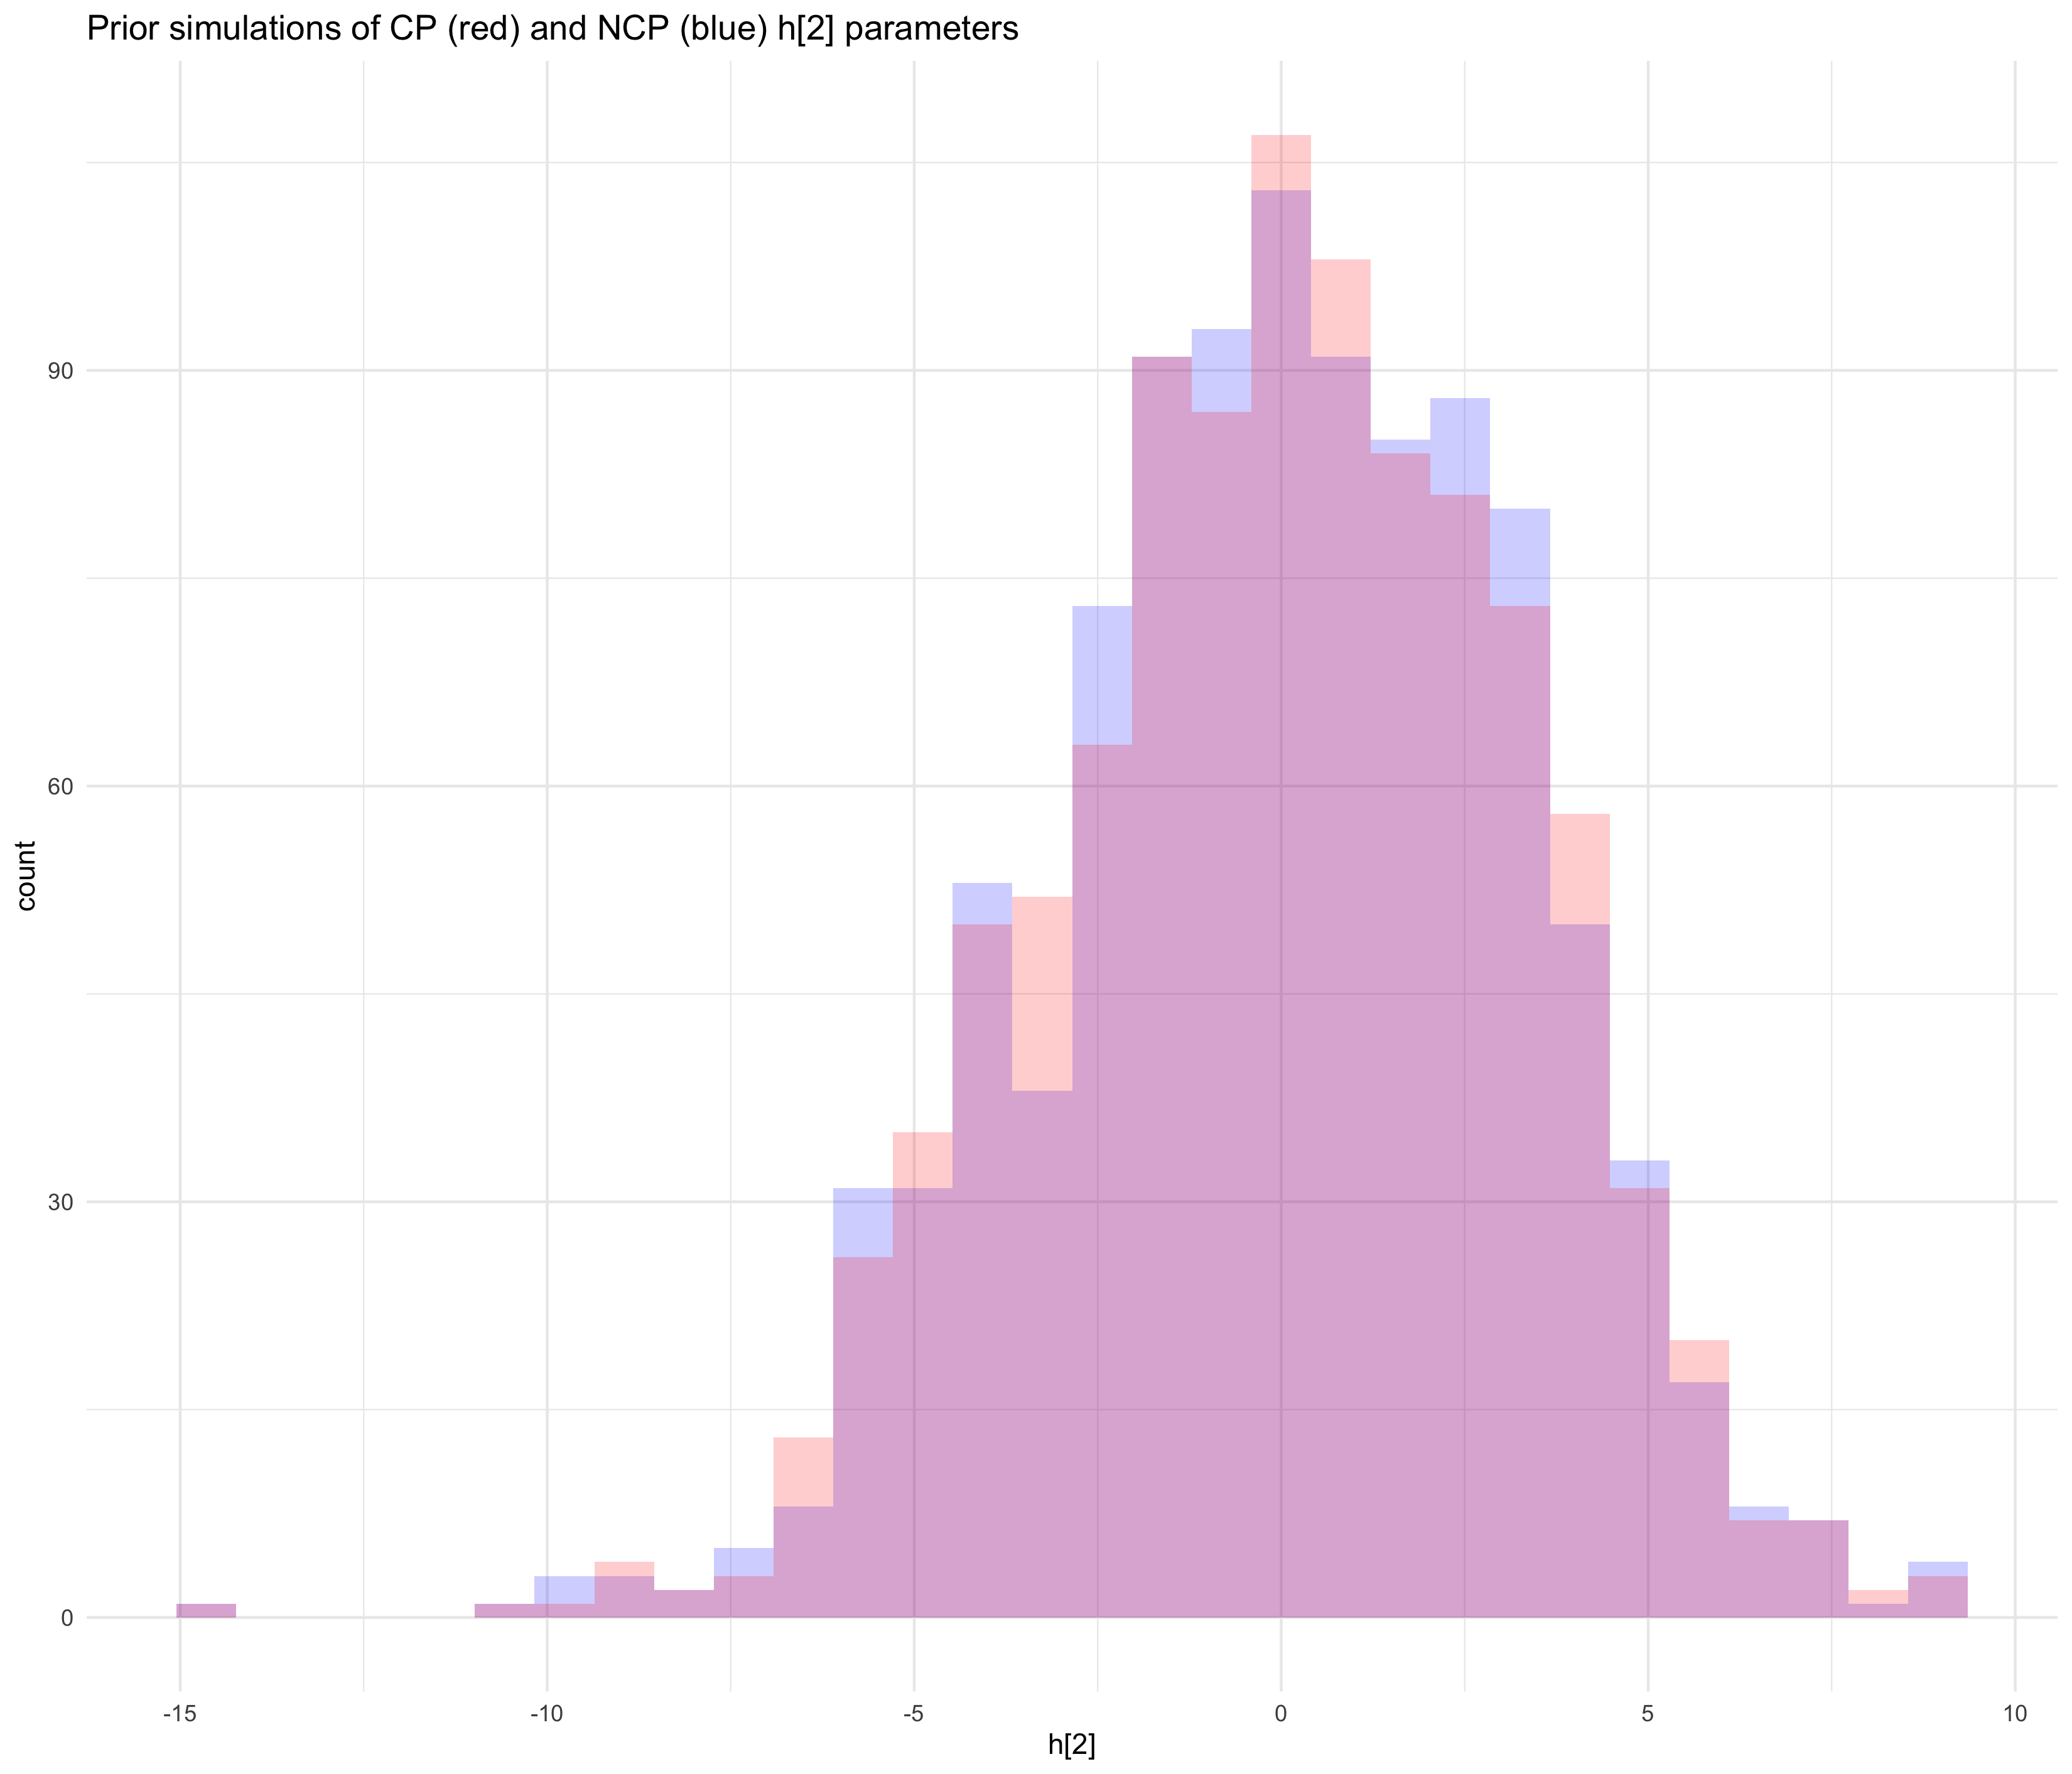
\includegraphics[scale=0.1]{ppc_h2.png}
        %     \caption{Prior predictive samples of second state variable}
        % \end{figure}
        
        % Emphasise here that different paramterisations of the models are the same model
        % Use a prior predictive check from both paramterisations show that the results are
        % the same

\section{Results}

    \subsection{Hamiltonian Monte Carlo}

    \subsection{Gaussian Mixture Approximation}

    \subsection{Reweigthing rank statistics of Gaussian Mixture}

\section{Discussion}

\subsection{Limitations}

\section{Conclusion}

\newpage

% \bibliographystyle{apa} % Econometrica referencing
\bibliography{references}

\end{document}
